        Die Rasterisierung spielt in konventionellen Bilderzeugungsverfahren eine große Rolle. 
        Zu Beginn der Rasterisierung haben wir die Eckpunkte der bereits verarbeiteten, transformierten, projizierten Geometrie mit möglichen
        Beleuchtungsinformationen aus den vorherigen Berechnungen vorliegen (weiterführende Literatur zu der modernen
        Renderingpipeline \cite{akenine2018real}). 
        Mit Hilfe der Rasterisierung wird nun die Farbe jedes einzelnen Pixels bestimmt. Es ist also die Aufgabe der Rasterisierung herauszufinden, 
        welche Geometrie welchen Pixel zu welchen Anteil bedeckt und wie die Shading Informationen zur Farbgebung des Pixels beitragen. 
        Aufgrund dieser Vorgehensweise spricht man auch von einem objektbasierten Bilderzeugungsverfahren.

        \begin{figure}[H]
            \centering
            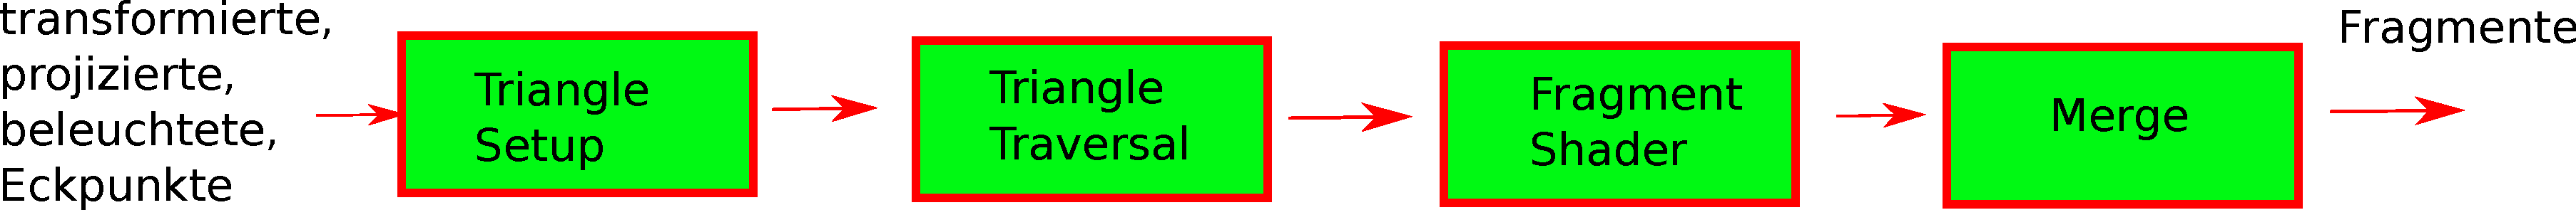
\includegraphics[width=\linewidth]{content/PathTracer/Bilder/Rasterisierung.pdf}
            \caption{Ablauf der Rasterisierung}
            \label{pic:Rasterisierungsablauf}
        \end{figure}

        
        Zuallererst befindet man sich im \nameref{pic:Rasterisierungsablauf} beim \textit{Triangle Setup}. Unbeeinflussbar vom Programmierer werden hier Daten berechnet, welche zur Pixeleinfärbung
        benötigt werden. So werden viele zuvor per Eckpunkt berechnete Werte interpoliert (Beleuchtung, Tiefe). Beim darauffolgenden \textit{Triangle Traversal} werden
        die wichtigen Fragmente erzeugt. Dieser Schritt bestimmt diejenigen Pixel, welche innerhalb des Dreiecks liegen und erzeugt darauf hin die Fragmente für dieses
        Dreieck anhand der zuvor berechneten/interpolierten per Dreieck Informationen. Als freiprogrammierbare Shadereinheit können im \textit{Fragment Shader}
        vom Programmierer weitere Berechnungen vorgenommen werden. Dazu zählt eine pro Pixel Beleuchtungsberechnung (Phong Shading).
        Im darauffolgenden Schritt wird mit dem Z-Buffer auf Sichtbarkeit geprüft. Die Ausgabe kann in mehrere verschiedene \textit{render targets}
        geschrieben und somit ein \textit{GBuffer} erzeugt werden. In einem ersten Schritt speichert man Informationen
        über das Material/Position vom Objekt in verschiedene \textit{render targets}. In einem zweiten Durchlauf kann man nun die Beleuchtung und einige andere 
        Effekte sehr effektiv berechnen.  
        Das abschließende nicht komplett freiprogrammierbare, aber hoch konfigurierbare \textit{Merging} hat eine besondere Aufgabe beim Abspeichern der Farbe für
        jeden Pixel im color Buffer. Zur Bestimmung der aktuellen Farbe wird nun auch das Problem der 
        Sichtbarkeit von Objekten angegangen. Zu den Z-Werten, welche wir als Tiefe beim Viewport Transform gespeichert haben, gibt
        es hier Zugang zum Depth/Z-Buffer. Dieser Z-Buffer speichert anfangs überall den Wert inf. Beim Durchlauf der Geometrie wird nun jeweils für jeden Pixel,
        der die Geometrie bedeckt der color und depth buffer wie folgt aktualisiert: Ist der verglichene Tiefenwert des vom Objekt erzeugten Fragment kleiner als der Wert
        im Tiefenbuffer für den betroffenen Pixel, so schreibt er diesen Tiefenwert in den Z-Buffer und auch der color Buffer mit der Fragmentfarbe aktualisiert.
        Falls nicht passiert nichts und das nächste Primitiv bzw. Fragment wird betrachtet (Szene ohne semitransparente Objekte!). Haben wir semitransparente Objekte, so 
        müssen wir zuerst die Szene wie beschrieben ohne diese Primitive zeichnen, alle semitransparenten Primitive nach ihrer Tiefe ordnen und in dieser Reihenfolge 
        zu dem zuvor gerenderten Bild hinzufügen. Damit haben wir auch unsere Projektion vollzogen, welche wir zuvor vorbereitet 
        haben(Weglassen der z-Komponente).\par 
        
        \subsection{Beschränktheit}
        \label{sec:Rasterisierung:Beschränktheit}
        
        
        \begin{figure}[H]
            \centering
            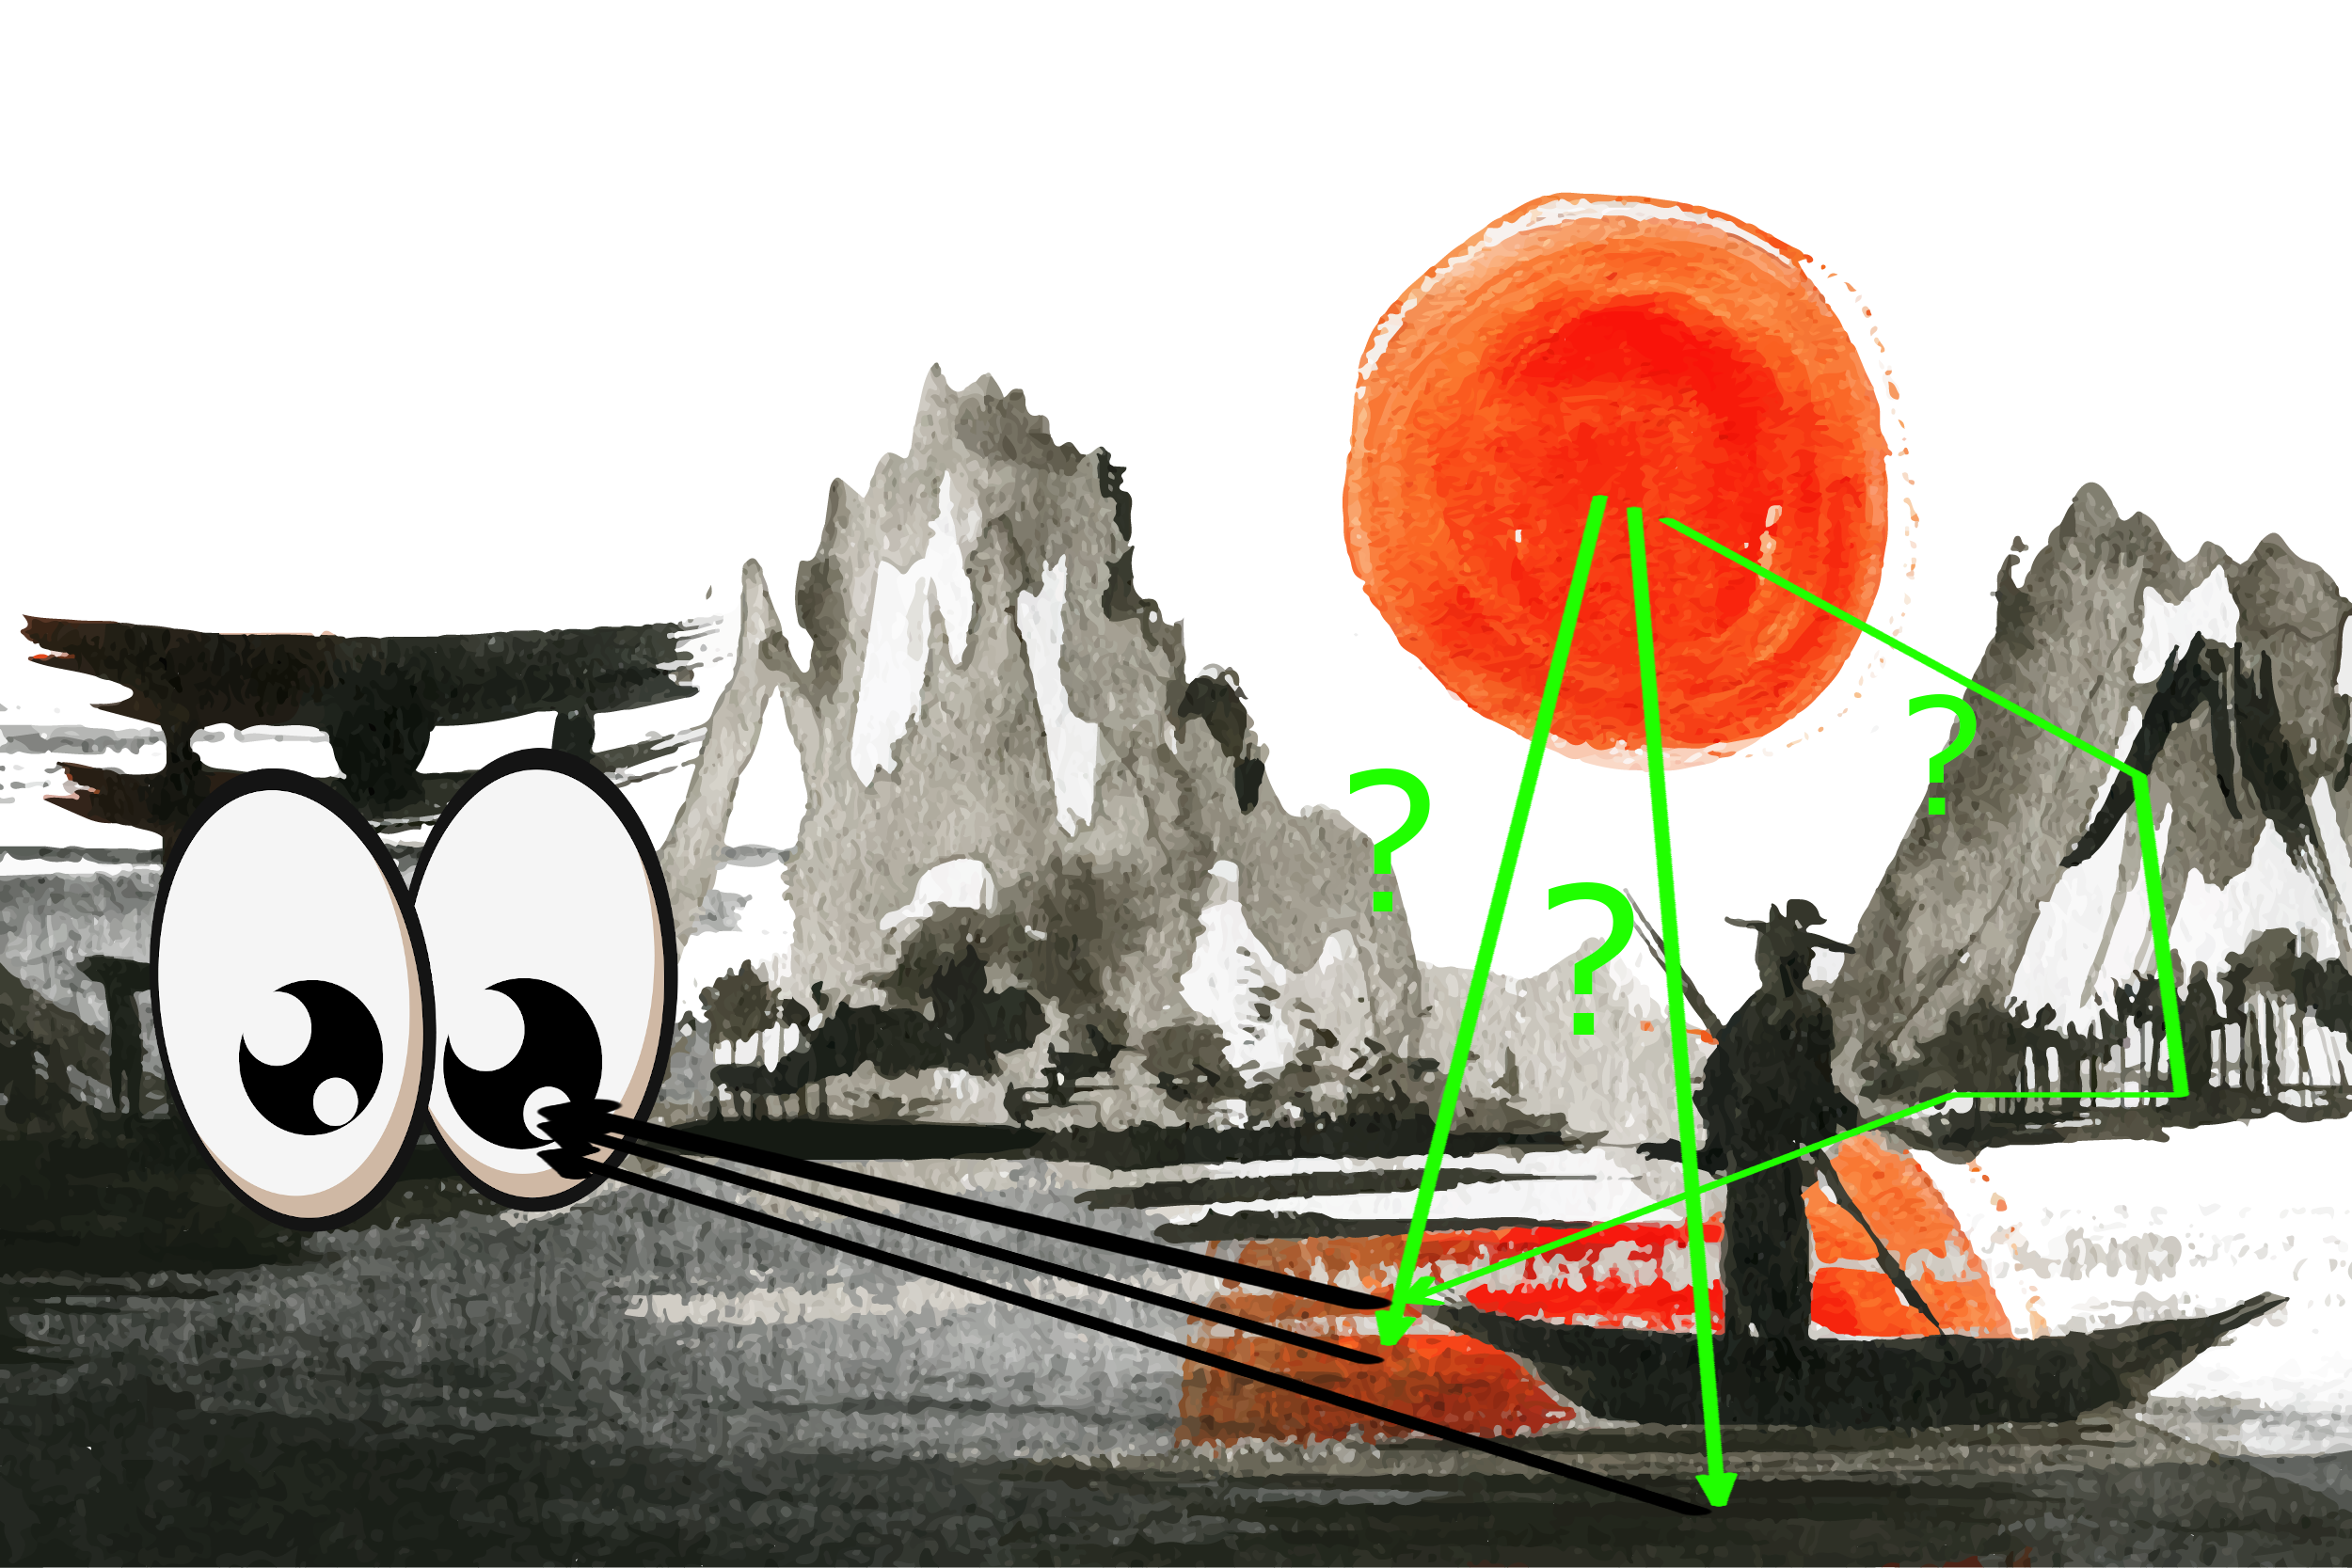
\includegraphics[width=\linewidth]{content/PathTracer/Bilder/RasterizerGuide.png}
            \caption{Ablauf der Rasterisierung}
            \label{pic:RasterizerGuide}
        \end{figure}

        Ihre bisherige weite Verbreitung hatte die Rasterisierung der Objektorientierung zu verdanken: massives paralleles Arbeiten, Ignorieren von (großen) leeren Bereichen und
        Ausnutzen von Cachekohärenzen gehören zu den Eigenschaften, welche die enorme effiziente, schnelle Abarbeitung bzw. (relativ) geringe aufzuwendende Rechenleistung begründen.
        Jedoch liegt in ihr auch die Crux.
        Die Abbildung der Farbe eines Geometrie/Dreiecks auf einen Pixel simuliert
        den physikalischen Lichttransport nicht korrekt! Die physikalische Optik lehrt uns das Verfolgen von weiteren (sekundären) Strahlen abseits des Primärstrahls, der von 
        Sichtebene zum Objekt verläuft und durch die Rasterisierung im Gegensatz zu den Sekundärstrahlen abgedeckt wird. Abbildung \ref{pic:RasterizerGuide} verdeutlicht das 
        Problem der Objektorientierung und deren Problem mit Sekundärstrahlen. So können Effekte, welche diese Sekundärstrahlen involvieren, 
        entweder nicht oder nur (unzureichend befriedigend) dargestellt werden (so in \ref{pic:RasterizerGuide} Spiegelungen, Schatten und Pfade mit größerer Pfadlänge). \par

        Die enormen Leistungsanforderungen von Technologien, welche diesen physikalisch korrekten Lichttransport möglich machen, haben Sie bisher für Echtzeitanwendungen ausgeschlossen.
        In heutigen modernen Grafikprogrammierschnittstellen (Vulkan, DirectX) jedoch befindet sich Raytracing-Funktionalität, welche auf Hardwareseite unterstützt wird.
        Diese Unterstützung erlaubt neuerdings effizientere image-ordered Bilderstellungen in Echtzeit.  
        Aktuelle Bemühungen gehen nun daran Strahlenerzeugung und Rasterisierung zu kombinieren. \cite{Barre-Brisebois2019} stellte
        mit dem Spiel \textit{PICA PICA} eine solche Rendering-Pipeline vor, welche mithilfe von Path Tracing\ref{ch:Content1:sec:Path Tracer} arbeitet. Dabei wird der G-Buffer
        (Texturen die Position, Normalen, Belichtung eines Bildes speichern) noch über Rasterisierung berechnet. Direkten Schatten kann man 
        rastern oder durch das Verschießen von Strahlen bekommen. Diese Option verspricht eine Anpassungsfähigkeit der Pipeline nach Leistungsfähigkeit der Hardware. Ähnlich können nun
        Reflexionen, Global Illumination, Ambient Occlusion und Transmission durch Verschießen von Strahlen oder auf Compute Shader ausgeführt werden (wieder je nach 
        Hardwareleistung). Einzig direkte Beleuchtung sowie Post-Processing Effekte laufen nur über Compute-Shader. \par

        Wir wollen diesen Ansatz in dieser Arbeit aufnehmen. Berechnung des \textit{GBuffer}'s mit Hilfe von Rasterisierung und globale Beleuchtung durch 
        einen \nameref{ch:Content1:sec:Path Tracer} erreichen. Da trotz hardwarebeschleunigtes Strahlenverschießen unsere Anzahl an Strahlen beschränkt ist, 
        beschäftigen wir uns innerhalb dieser Arbeit mit einem \nameref{ch:Temporaler Algorithmus}, der die visuelle Qualität nicht durch Verschießen von mehr Strahlen, 
        sondern durch eine zeitlich stabile \nameref{ch:Content1:sec:blue noise} Fehlerverteilungen im Bildraum erreicht.